\chapter{引导与可控生成}\label{ch:guidance}
扩散模型是强大的生成框架。在无条件设置下，目标是学习 $p_{\text{data}}(\rvx)$ 并在没有外部输入的情况下生成样本。

然而，许多应用需要 \emph{ 条件生成 }，其中输出满足用户指定的标准。这可以通过引导无条件模型或直接学习条件分布 $p_0(\rvx | \rvc)$ 来实现，条件 $\rvc$（例如标签、文本描述或草图）指导该过程。

本章建立在条件分数的原理视图的基础上，它分解为 \emph{ 非条件方向 } 和 \emph{ 指导方向 }，在保持真实性的同时将样本推向条件。我们解释了为什么指导是必要的，展示了条件分数如何作为控制的统一界面，并调查了近似或替换指导术语的方法。然后，我们区分 \emph{control}（满足条件）和 \emph{alignment}（满足条件下的人类偏好），并描述如何将偏好合并到同一框架中。最后，我们讨论在没有额外奖励模型的情况下直接优化偏好（即，一个学习评分器，为与人类偏好更一致的输出分配更高的值）。


\chapterlearning{

  \item 了解调节如何修改扩散采样期间使用的速度场；

  \item 导出分类器引导和无分类器引导背后的关键思想，并了解引导强度如何控制调节；

  \item 了解免训练引导如何使用特定于任务的损失或测量模型来引导预训练的扩散模型，包括逆问题；

  \item 将精确条件采样与替代引导动力学及其固定时间倾斜密度解释区分开来；

  \item 了解基于偏好的对齐（从 RLHF 到 DPO 和 Diffusion-DPO）如何进一步重塑条件生成模型以实现首选输出。

}{ 本章假设 Score SDE/PF-ODE 图片来自 \Cref{ch:score-sde,ch:all-equivalent}。主要对可控发电感兴趣的读者可以将后面的偏好调整材料视为第二遍。}





\clearpage
\newpage

\section{序言}\label{sec:prologue-guidance}\begin{figure}[th!]
    \centering
    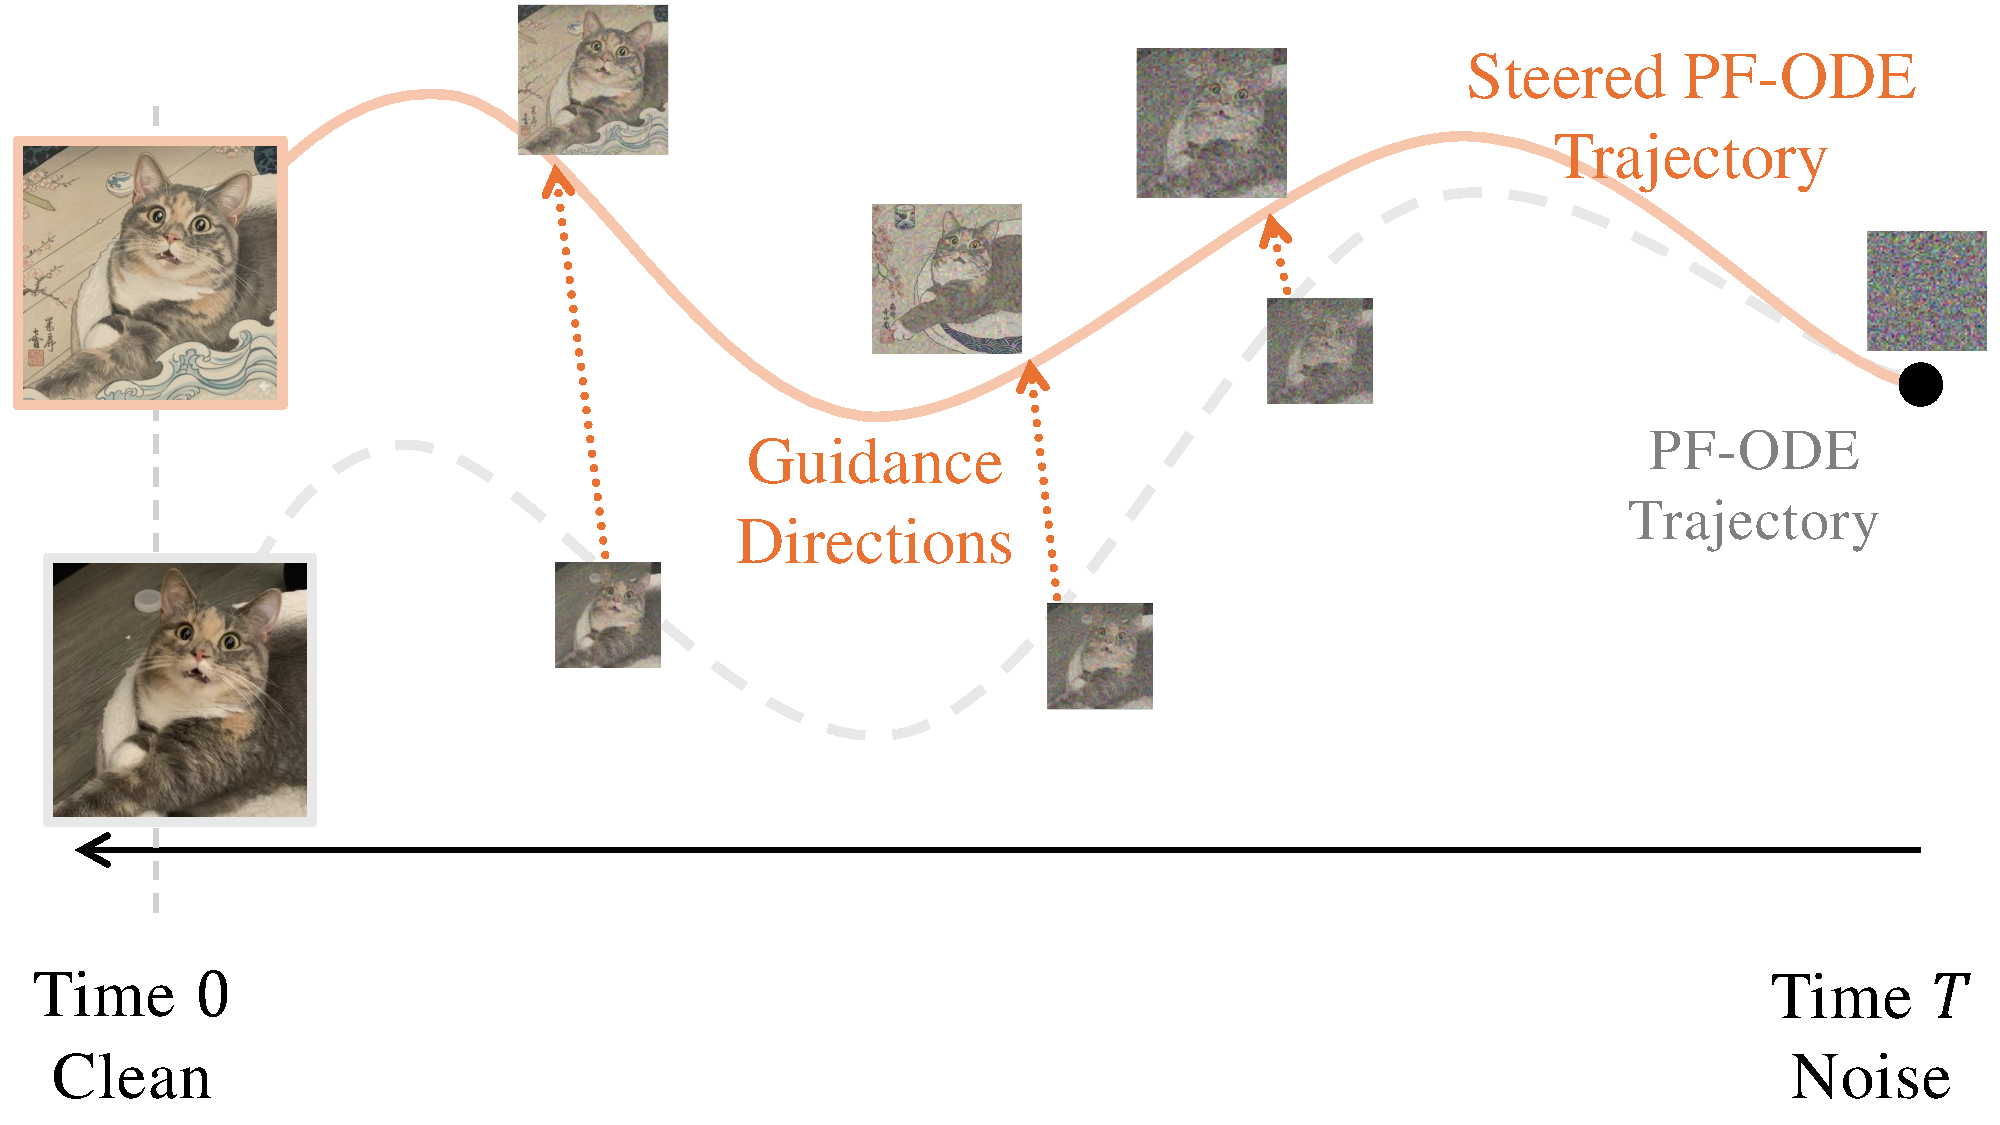
\includegraphics[width=\linewidth]{Images/PartC/guidance.pdf}
\caption{\textbfs{ 定向扩散采样示意图。}
反时 PF-ODE 采样从右侧的纯噪声 ($t = T$) 开始，逐渐演变为左侧的干净样本 ($t = 0$)。
在此过程中，由 $w_t$ 加权的时间相关引导方向修改无条件分数字段并将轨迹引导至所需属性（日本绘画风格），同时样本从粗到细的细节逐渐细化。
\figcredit{由作者创建。}}
    \label{fig:guidance}
\end{figure}


扩散模型的生成过程以从粗到细的方式进行，为可控生成提供了灵活的框架。每一步都会去除少量噪音，样本变得更加清晰，逐渐揭示更多结构和细节。此属性可以控制生成过程：通过向学习的、与时间相关的速度场添加指导项，我们可以引导生成轨迹以反映用户意图。

扩散模型中基于指导的采样的原则基础是条件分数的贝叶斯分解。对于每个噪声级别 $t$，
\begin{mdframed}
\begin{align}
\nabla_{\rvx_t}\log p_t(\rvx_t |\rvc)
=
\underbrace{\nabla_{\rvx_t}\log p_t(\rvx_t)}_{\text{unconditional direction}}
+
\underbrace{\nabla_{\rvx_t}\log p_t(\rvc |\rvx_t)}_{\text{guidance direction}}.
\label{eq:guidance_bayes}
\end{align}
\end{mdframed}
这个恒等式表明，通过添加指导项可以获得精确的条件反向动力学
$\nabla_{\rvx_t}\log p_t(\rvc|\rvx_t)$ 在无条件分数之上。我们稍后会看到分类器引导~\citep{dhariwal2021diffusion}直接估计这个术语，
无分类器引导~\citep{ho2021classifier}将其隐式估计为联合学习的条件分数和无条件分数之间的差异，
更通用的免训练方法可能会使用特定于任务的替代指导方向。

有了精确的条件分数，PF-ODE 就变成
\begin{align}\label{eq:condition_prob_ode}
\begin{aligned}
    \frac{\diff \mathbf{x}(t)}{\diff t} &= f(t)\mathbf{x}(t) - \frac{1}{2} g^2(t) \underbrace{\nabla_{\rvx_t} \log p_t(\rvx(t) |\rvc)}_{\text{conditional score}} \\
    &= f(t)\mathbf{x}(t) - \frac{1}{2} g^2(t) \Big[ \nabla_{\rvx_t} \log p_t(\rvx(t)) + \nabla_{\rvx_t} \log p_t(\rvc |\rvx(t)) \Big].
\end{aligned}
\end{align}
通过精确的分数和精确的积分，这些动态就会恢复
$p_0(\rvx_0|\rvc)$ 初始化时从对应的终端边缘开始
$p_T(\rvx_T|\rvc)$。在标准扩散结构中，终端噪声
选择使得 $p_T(\rvx_T|\rvc)$ 与通常的近似匹配
条件无关先验。

为了清楚起见，我们在分数预测中制定了下面的讨论。自从
标准 $\rvx$-、$\beps$-、分数-和 $\rvv$-预测参数化是
无论这些转换在哪里，都通过与时间相关的线性变换相关
定义明确，相同的指导修正可以用其他形式表示
使用 \Cref{eq:predictions-equivalence} 中的关系进行参数化。\paragraph{引导方向的实例.}
\begin{enumerate}[leftmargin=*]
\item \textbfs{分类器引导 (CG).} 在 \Cref{sec:cg} 中，分类器引导 (CG) 训练时间条件分类器
$p_{\bpsi}(\rvc | \rvx_t, t)$ 上的噪声数据 $\rvx_t$（通过破坏
清洁 $t$ 级别的标记样品）。在采样时，其输入梯度
提供指导术语：
\[
\nabla_{\rvx_t}\log p_{\bpsi}(\rvc | \rvx_t, t)
 \approx  \nabla_{\rvx_t}\log p_t(\rvc | \rvx_t),
\]
然后将其添加到无条件分数 ~\citep{dhariwal2021diffusion} 中。
\item \textbfs{Classifier-Free Guidance (CFG).} 在\Cref{sec:cfg}中，CFG直接训练单个条件模型
\[
\rvs_{\bphi}(\rvx_t,t,\rvc) \approx \nabla_{\rvx_t}\log p_t(\rvx_t|\rvc),
\]
其中，无条件模型是通过在训练步骤的一部分中随机用特殊的空标记替换条件来联合学习的。
\item \textbfs{免训练（替代）指导.}
在标准前向噪声结构下，我们首先画出
$(\rvx_0,\rvc)\sim p_{\mathrm{data}}$ 然后取样
$\rvx_t\sim p_t(\cdot|\rvx_0)$，其中前向内核不依赖
另外在 $\rvc$ 上。因此
$\rvc\perp\rvx_t\mid\rvx_0$\footnote{
确实，
\[
p_t(\rvc|\rvx_t)
=
\int
p(\rvc,\rvx_0|\rvx_t)\,\mathrm d\rvx_0
=
\int
p(\rvc|\rvx_0,\rvx_t)\,
p(\rvx_0|\rvx_t)\,\mathrm d\rvx_0.
\]
因为标准前向内核满足
$p_t(\rvx_t|\rvx_0,\rvc)=p_t(\rvx_t|\rvx_0)$，
我们有
$p(\rvc|\rvx_0,\rvx_t)=p(\rvc|\rvx_0)$,
产生下面的表达式。
}。
因此，
\[
p_t(\rvc|\rvx_t)
=
\int
p(\rvc|\rvx_0)\,
p(\rvx_0|\rvx_t)\,
\mathrm d\rvx_0.
\]
这种后验平均值通常很棘手，无需训练即可激励
相反，构建特定于任务的替代指导方向的方法。

在 \Cref{subsec:tfg} 中，免训练（基于损失）指导避免了评估
直接条件似然 $p_t(\rvc|\rvx_t)$。相反，它从一个
现成的损耗 $\ell(\rvx_t,\rvc;t)$ 用于测量电流的好坏
样本满足要求的条件，损失越小越好
协议。根据该损失，我们定义了正 \emph{ 指导势}
\[
\rvh_t(\rvx_t;\rvc)
:=
\exp\big(-\tau\,\ell(\rvx_t,\rvc;t)\big),
\qquad \tau>0.
\]
因此，损耗较低的样本会获得较大的潜在值。我们表示
对应\emph{引导方向}由
\[
\mathcal{G}_t(\rvx_t,\rvc)
:=
\nabla_{\rvx_t}\log \rvh_t(\rvx_t;\rvc)
=
-\tau\nabla_{\rvx_t}\ell(\rvx_t,\rvc;t).
\]

分类器引导自然地适合同一张图片。在人口方面
水平，其指导潜力为
\[
\rvh_t(\rvx_t;\rvc)
=
p_t(\rvc|\rvx_t),
\]
在实践中由学习到的分类器近似
$p_{\bpsi^\times}(\rvc|\rvx_t,t)$。等价地，学习到的分类器
对应于损失
\[
\ell(\rvx_t,\rvc;t)
=
-\log p_{\bpsi^\times}(\rvc|\rvx_t,t),
\qquad \tau=1.
\]


\end{enumerate}

在人口层面，以上三种结构具有相同的加法
指导模板。赋予积极的潜力
$\rvh_t(\rvx_t;\rvc)$ 和指导强度 $w_t\geq0$，定义指导分数
领域
\begin{align}
\rvs^{\mathrm{guide}}(\rvx_t,t,\rvc;w_t)
:=
\nabla_{\rvx_t}\log p_t(\rvx_t)
+
w_t\mathcal{G}_t(\rvx_t,\rvc).
\label{eq:generic-guided-score}
\end{align}
对于基于损失的指导，
$\mathcal{G}_t(\rvx_t,\rvc)
=-\tau\nabla_{\rvx_t}\ell(\rvx_t,\rvc;t)$。
对于准确的分类器引导，
$\mathcal{G}_t(\rvx_t,\rvc)
=\nabla_{\rvx_t}\log p_t(\rvc|\rvx_t)$;无分类器引导表示
通过差异来实现相同的人口引导方向
有条件分数和无条件分数。

在每个固定时间$t$，\Cref{eq:generic-guided-score}，每当
可归一化，倾斜密度的分数
\[
\widetilde p_t^{\mathrm{tilt}}(\rvx_t|\rvc)
\propto
p_t(\rvx_t)\rvh_t(\rvx_t;\rvc)^{w_t}.
\]
这给出了有用的能量解释：基础密度有利于样本
由扩散模型支持，而潜力将它们重新加权
所需的条件。在实践中，相应的学习或代理版本
\Cref{eq:generic-guided-score} 被插入到逆时动态中。
重要的是，上面的倾斜密度只是一个固定时间的解释：
家人
$\{\widetilde p_t^{\mathrm{tilt}}(\cdot|\rvc)\}_t$
不需要与引导采样器生成的边缘一致。
因此，对于通用损失或指导时间表，整合指导
从 $T$ 到 $0$ 的 PF-ODE 通常不会生成分布式样本
根据 $\widetilde p_0^{\mathrm{tilt}}(\cdot|\rvc)$。
这种解释成立所需的额外跨时间一致性
在 \Cref{subsec:guided-marginal-path} 中进行了讨论。


引导对采样轨迹的影响如图所示
\Cref{fig:guidance}。同样的原理也可以应用在
已经有条件的模型，允许额外的控制信号来修改其
采样动态。












\paragraph{从控制到通过直接偏好优化更好地对齐。}

强控制可以是有条件的，但不是偏好的：样本可以满足
条件信号（例如提示）但偏离了人类的实际情况
更喜欢。我们通过将条件目标倾斜 $t=0$ 来形式化这一点
偏好等级：
\[
\widetilde p_0^{\mathrm{tilt}}(\rvx_0|\rvc)
\propto
p_0(\rvx_0|\rvc)
\exp\bigl(
\lambda_{\mathrm{pref}} r(\rvx_0,\rvc)
\bigr),
\qquad
\lambda_{\mathrm{pref}}>0,
\]
其中 $r(\rvx_0,\rvc)$ 是干净样本的标量对准评级
$\rvx_0$和条件$\rvc$，数值越大表示越强
偏好，$\lambda_{\mathrm{pref}}$ 控制的强度
偏好重新加权。在后面介绍的KL正则化公式中，
优化器采用这种形式，以参考策略为基础
分布和$\lambda_{\mathrm{pref}}=1/\beta$。









































实现这种可操纵性的现有方法通常会收集模型生成相对质量的人类标签，并通常通过人类反馈（RLHF）的强化学习来微调条件扩散模型以符合这些偏好。然而，RLHF 是一个复杂且通常不稳定的过程：它首先拟合奖励模型来捕获人类偏好，然后通过强化学习微调条件扩散模型，以最大化估计的奖励，同时限制政策与原始模型的偏差。

这自然会提出一个问题：\emph{ 我们可以完全删除奖励模型训练阶段吗？} 我们通过 Diffusion-DPO~\citep{wallace2024diffusion} 来解决这个问题，它是最初为大型语言模型开发的直接偏好优化 ~\citep{rafailov2023direct} 的改编版。如 \Cref{sec:rlhf-dpo} 中所述，Diffusion-DPO 直接从成对选择中学习偏好倾斜，因此条件扩散模型经过微调以适应偏好，而无需单独的奖励模型。







































































































\clearpage
\newpage


\section{分类器引导}\label{sec:cg}

\subsection{分类器引导的基础}
让 $\rvc$ 表示从分布中提取的条件变量 $p(\rvc)$，例如类标签、标题或其他辅助信息。我们的目标是从中抽取样本 $p_0(\rvx | \rvc)$。在基于扩散的条件生成中，我们通过运行时间边缘为的逆时动力学来实现这一目标 $p_t(\cdot | \rvc)$。这些动态的漂移取决于条件分数
\[
\nabla_{\rvx_t}\log p_t(\rvx_t | \rvc), \quad t \in [0,T].
\]
因此是标准且有效的路线\footnote{原则上可以获得 $p_0(\rvx | \rvc)$ 来自无条件生成器，通过拒绝或重要性采样，如果 $p(\rvc | \rvx)$ 可用且经过良好校准。这对于高维或稀有条件来说很少实用。} 是估计这个数量。基于贝叶斯规则的一个基本见解是条件分数可以分解为：
\begin{align}
\nabla_{\rvx_t} \log p_t(\rvx_t | \rvc) 
&= \nabla_{\rvx_t} \log \left( \frac{p_t(\rvx_t)   p_t(\rvc | \rvx_t)}{p(\rvc)} \right) \nonumber \\
&= \nabla_{\rvx_t} \log p_t(\rvx_t) + \nabla_{\rvx_t} \log p_t(\rvc | \rvx_t) - \nabla_{\rvx_t} \log p(\rvc) \nonumber \\
&= \underbrace{\nabla_{\rvx_t} \log p_t(\rvx_t)}_{\text{unconditional score}} 
+ \underbrace{\nabla_{\rvx_t} \log p_t(\rvc | \rvx_t)}_{\text{classifier gradient}}, \label{eq:cg_bayes}
\end{align}
哪里 $p_t(\rvc | \rvx_t)$ 表示概率 $\mathbf{c}$ 条件为 $\mathbf{x}_{t}$ 预测条件 $\rvc$ 来自噪声输入 $\rvx_t$ 当时 $t$。这个分解\footnote{在最后一个恒等式中，
$\nabla_{\rvx_t}\log p(\rvc)=0$ 因为 $p(\rvc)$ 不依赖于
$\rvx_t$.} 激励 \emph{分类器引导} （CG）提出的方法
\citet{dhariwal2021diffusion}。为了将群体恒等式与实践中使用的学习分类器分开，首先考虑预言数量。对于指导规模 $\omega\geq0$，在每个固定时间定义 $t$
\begin{align}
\widetilde p_t^{\mathrm{CG},\omega}(\rvx_t|\rvc)
\propto
p_t(\rvx_t)p_t(\rvc|\rvx_t)^\omega.
\label{eq:cg-density-omega}
\end{align}
其分数为
\begin{align}
\rvs^{\mathrm{CG}}(\rvx_t,t,\rvc;\omega)
&:=
\nabla_{\rvx_t}
\log\widetilde p_t^{\mathrm{CG},\omega}(\rvx_t|\rvc)
\nonumber\\
&=
\nabla_{\rvx_t}\log p_t(\rvx_t)
+
\omega\nabla_{\rvx_t}\log p_t(\rvc|\rvx_t).
\label{eq:cg_omega}
\end{align}
因此 $\omega$ 缩放分类器引导方向。当 $\omega=1$，贝叶斯规则给出
$\widetilde p_t^{\mathrm{CG},1}(\rvx_t|\rvc)=p_t(\rvx_t|\rvc)$, 和
\Cref{eq:cg_omega} 恢复精确的条件分数。对于一般
$\omega$, $\widetilde p_t^{\mathrm{CG},\omega}$ 提供引导场的固定时间缓释解释；它是否也形成引导采样器的边缘路径在
\Cref{subsec:guided-marginal-path}。标量 $\omega \ge 0$ 调节分类器的影响：
\begin{itemize}
    \item $\omega = 1$: 恢复真实的条件分数 $\nabla_{\rvx_t} \log p_t(\rvx_t |\rvc)$.
    \item $\omega > 1$：放大分类器信号，通常会提高条件保真度（通常以牺牲多样性为代价）。
    \item $0 \le \omega < 1$：降低分类器信号的权重，通常会增加样本多样性，同时削弱调节。
\end{itemize}

\paragraph{CG 中的实用近似。}
在实践中，CG 是一种免训练的方法（w.r.t.\ 扩散模型），用于引导预训练的无条件扩散模型，
\[
\rvs_{\bm{\phi}^\times}(\rvx_t ,t) \approx \nabla_{\rvx_t} \log p_t(\rvx_t).
\]
CG仅在采样时应用，而不修改扩散模型本身。为了实现这一点，依赖于时间的分类器 $p_{\bpsi}(\rvc |\rvx_t,t)$ 单独训练以预测状况 $\rvc$ 来自噪声输入 $\rvx_t$ 不同噪音水平 $t$。通过最小化交叉熵损失以标准方式训练分类器：
\begin{align}
\mathbb{E}_{t \sim \mathcal{U}[0,T], (\rvx, \rvc) \sim p_{\text{data}},  \bm{\epsilon} \sim \mathcal{N}(\mathbf{0}, \mathbf{I})}
\Big[ -\log p_{\bpsi}(\rvc | \rvx_t,t) \Big],
\end{align}
哪里 $(\rvx,\rvc)\sim p_{\text{data}}$ 表示配对标记数据，并且 $\rvx_t = \alpha_t \rvx + \sigma_t \bm{\epsilon}$ 是此时的噪声输入 $t$。分类器必须在噪声级别上进行训练，并且通常接收 $t$，或等效的噪声级别表示，作为输入，以便它可以近似
$p_t(\rvc|\rvx_t)$ 整个扩散路径。训练后，分类器提供分数作为真实似然梯度的替代：
\[
\nabla_{\rvx_t} \log p_{\bpsi^\times}(\rvc |\rvx_t,t) \approx \nabla_{\rvx_t} \log p_t(\rvc |\rvx_t).
\]


\subsection{用 CG 进行推理}
在推理时，学习到的分类器梯度
$\nabla_{\rvx_t}\log p_{\bpsi^\times}(\rvc|\rvx_t,t)$ 添加到无条件分数估计中并按比例缩放 $\omega$，产生对 oracle 字段的学习近似 \Cref{eq:cg_omega}:
\begin{align*}
\rvs^{\mathrm{CG}}_{\mathrm{model}}(\rvx_t,t,\rvc;\omega)
:=
\underbrace{\rvs_{\bm{\phi}^\times}(\rvx_t,t)}_{\text{uncond.\ direction}}
+
\omega
\underbrace{\nabla_{\rvx_t}\log
p_{\bpsi^\times}(\rvc|\rvx_t,t)}_{\text{guidance direction}}
\approx
\rvs^{\mathrm{CG}}(\rvx_t,t,\rvc;\omega).
\end{align*}
反时 SDE 或 PF-ODE 中的无条件分数估计被替换为
$\rvs^{\mathrm{CG}}_{\mathrm{model}}(\rvx_t,t,\rvc;\omega)$，从而将生成轨迹转向与条件相符的样本 $\rvc$.



\subsection{优点和局限性}

CG 为条件生成提供了一种简单而灵活的机制，允许通过以下方式显式控制条件的强度 $\omega$。它可以与任何预先训练的无条件扩散模型一起使用，只需要一个额外的分类器进行调节。然而，该方法有明显的局限性：
\begin{itemize}
    \item \textbfs{训练费用：} 分类器必须经过训练才能在所有噪声级别上运行，这在计算上是昂贵的。
    \item \textbfs{稳健性：} 分类器必须能够很好地泛化到严重损坏的输入 $\rvx_t$，特别是对于大型 $t$，这可能具有挑战性。
    \item \textbfs{单独训练：} 由于分类器的训练独立于扩散模型，因此它可能无法与学习的数据分布完全一致。
\end{itemize}

\clearpage
\newpage

\section{无分类器引导}\label{sec:cfg}
\subsection{无分类器引导的基础}
\begin{figure}[th!]
    \centering
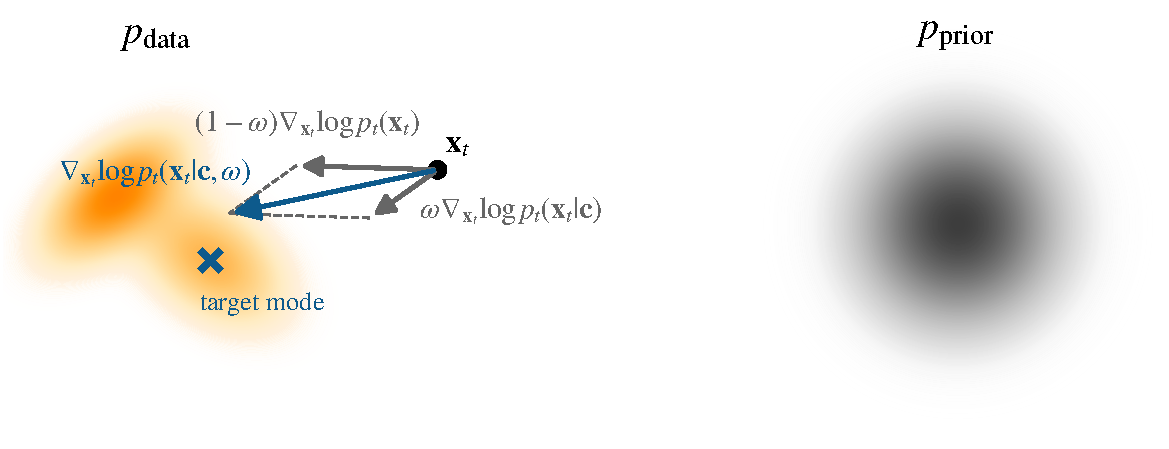
\includegraphics[width=\linewidth]{Images/PartB/classifier_guidance_v2.pdf}
\caption{\textbfs{ CFG.} 插图
引导方向是条件分数的线性组合
$\nabla_{\rvx_t}\log p_t(\rvx_t|\rvc)$ 和无条件分数
$\nabla_{\rvx_t}\log p_t(\rvx_t)$，由$\omega$控制。
对于 $0\leq\omega\leq1$，这会在两个方向之间进行插值；为了
$\omega>1$，它推断出超出条件分数的条件
方向。由此产生的场用于引导采样轨迹
调节信号。
\figcredit{由作者创建。}}
    \label{fig:cfg}
\end{figure}

\emph{无分类器引导} (CFG)~\citep{ho2021classifier}消除了需要
通过表达分类器引导来单独训练分类器
通过有条件和无条件分数来确定方向。贝叶斯规则给出
\begin{align}
\nabla_{\rvx_t}\log p_t(\rvc|\rvx_t)
=
\nabla_{\rvx_t}\log p_t(\rvx_t|\rvc)
-
\nabla_{\rvx_t}\log p_t(\rvx_t).
\end{align}
将此恒等式代入 \Cref{eq:cg_omega} 给出 oracle CFG 字段
\begin{align}\label{eq:cfg-model}
\rvs^{\mathrm{CFG}}(\rvx_t,t,\rvc;\omega)
&:=
\nabla_{\rvx_t}\log p_t(\rvx_t)
+
\omega
\left(
\nabla_{\rvx_t}\log p_t(\rvx_t|\rvc)
-
\nabla_{\rvx_t}\log p_t(\rvx_t)
\right)
\nonumber\\
&=
\omega
\underbrace{\nabla_{\rvx_t}\log p_t(\rvx_t|\rvc)}_{\text{conditional score}}
+
(1-\omega)
\underbrace{\nabla_{\rvx_t}\log p_t(\rvx_t)}_{\text{unconditional score}}.
\end{align}
有了精确的分数，\Cref{eq:cfg-model} 在代数上是相同的引导场
如 \Cref{eq:cg_omega}。在 $\omega=1$ 处，它简化为精确的条件
分数。对于其他引导优势，其固定时间倾斜密度
解释应与由
引导动力学，如所讨论的
\Cref{subsec:guided-marginal-path}。

超参数 $\omega$ 在控制条件信息的影响方面再次发挥着关键作用（我们采用 $\omega \ge 0$）：
\begin{itemize}
    \item 在 $\omega = 0$ 中，模型表现为无条件扩散模型，完全忽略调节。
    \item 在 $\omega = 1$ 中，模型使用条件分数，无需额外指导。
    \item 对于 $\omega > 1$，该模型更重视条件分数，而不是无条件分数，加强了与 $\rvc$ 的一致性，但通常会降低多样性。
\end{itemize}

\subsection{CFG}的训练和采样


\paragraph{通过CFG.}联合训练无条件和条件扩散模型
CFG 需要经过训练以支持条件和条件的扩散模型
无条件的预测。 CFG 没有训练两个单独的模型，而是使用
单个型号 $\rvs_{\bm{\phi}}(\rvx_t,t,\rvc)$ 并随机替换
在训练期间通过空标记 $\emptyset$ 调节输入：
\begin{itemize}
    \item 具有空输入，模型学习无条件预测
    $\rvs_{\bm{\phi}}(\rvx_t,t,\emptyset)$;
    \item 与原始条件，它学习条件预测
    $\rvs_{\bm{\phi}}(\rvx_t,t,\rvc)$。
\end{itemize}
零条件以 $p_\mathrm{uncond}$ 的概率使用，
用户指定的条件退出概率。完整的训练流程是
\Cref{alg:cfg_training} 中所示，以及标准无条件训练
\Cref{alg:no_cfg_training}。仅介绍指导重量$\omega$
在采样时，不是此训练目标的一部分。\begin{center}
\begin{minipage}[t]{0.48\textwidth}
  \begin{algorithm}[H]
  {\small
    {\small \caption{Uncond。 DM \label{alg:no_cfg_training} }}
    \begin{algorithmic}[1]
      \Repeat
        \State $\rvx \sim p_{\text{data}}(\rvx)$
        \State $t \sim \mathcal{U}[0, T]$
        \State $\bm{\epsilon} \sim \mathcal{N}(\mathbf{0}, \mathbf{I})$
        \State $\rvx_t = \alpha_t \rvx + \sigma_t \bm{\epsilon}$
        \State 采取梯度步骤：
        \Statex \quad $\nabla_{\bm{\phi}} \left\| \rvs_{\bm{\phi}}(\rvx_t, t) - \rvs \right\|^2$
      \Until{融合}
    \end{algorithmic}
    }
  \end{algorithm}
\end{minipage}
\hfill
\begin{minipage}[t]{0.48\textwidth}
  \begin{algorithm}[H]
      {\small
    {\small \caption{CFG 用于电导率。 DM \label{alg:cfg_training}}}
    \begin{algorithmic}[1]
      \Require \textcolor{orange}{$p_\mathrm{uncond}$：问题。无条件退出}
      \Repeat
        \State \textcolor{orange}{$(\rvx, \rvc) \sim p_{\text{data}}(\rvx, \rvc)$}
        \State \textcolor{orange}{$\rvc \gets \emptyset$ 有问题。 $p_\mathrm{uncond}$}
        \State $t \sim \mathcal{U}[0, T]$
        \State $\bm{\epsilon} \sim \mathcal{N}(\mathbf{0}, \mathbf{I})$
        \State $\rvx_t = \alpha_t \rvx + \sigma_t \bm{\epsilon}$
        \State 采取梯度步骤：
        \Statex \quad \textcolor{orange}{$\nabla_{\bm{\phi}} \left\| \rvs_{\bm{\phi}}(\rvx_t, t, \rvc) - \rvs \right\|^2$}
      \Until{融合}
    \end{algorithmic}
    }
  \end{algorithm}
\end{minipage}
\end{center}

\paragraph{带CFG的条件采样.}

一旦模型 $\rvs_{\bm{\phi}^\times}(\rvx_t,t,\rvc)$ 使用
算法~\ref{alg:cfg_training}，CFG形成学习引导场
\begin{align}\label{eq:cfg-model-nn}
\rvs_{\mathrm{model}}^{\mathrm{CFG}}(\rvx_t,t,\rvc;\omega)
&:=
\omega
\underbrace{\rvs_{\bm{\phi}^\times}(\rvx_t,t,\rvc)}_{\text{conditional score estimate}}
+
(1-\omega)
\underbrace{\rvs_{\bm{\phi}^\times}(\rvx_t,t,\emptyset)}_{\text{unconditional score estimate}}
\nonumber\\
&\approx
\rvs^{\mathrm{CFG}}(\rvx_t,t,\rvc;\omega).
\end{align}
采样期间，逆时 SDE 中的无条件分数估计或
PF-ODE 被替换为
$\rvs_{\mathrm{model}}^{\mathrm{CFG}}$。
因此，CFG 通过结合学习到的数据定义了一个修改后的采样域
有条件和无条件分数估计。

该配方可以通过调节 $\omega$ 来实现可控发电，
提供体能训练强度和训练后的简单权衡
样本多样性，无需单独训练的分类器或
无条件扩散模型。













\clearpage
\newpage



\section{免训练引导}
免训练引导修改了固定预训练的采样动态
使用外部条件、损耗或测量目标的扩散模型，
无需重新训练扩散模型本身。贝叶斯分解
\Cref{eq:guidance_bayes} 在分数空间中提供了有用的动机：指导
将条件相关的方向添加到无条件分数中。在实践中，
特定于任务的损失可用于构建对
预测的干净样本或采样期间使用的分数。

我们首先在\Cref{subsec:tfg}中介绍这两种通用形式。然后我们问
这种替代引导的动力学实际上会产生什么分布
\Cref{subsec:guided-marginal-path}，在转向代表之前
逆问题的免训练方法
\Cref{subsec:inverse-problem}。\paragraph{设置和符号.}
让 $\rvc$ 表示条件变量。我们假设可以访问预先训练的
扩散模型 $\rvs_{\bm{\phi}^\times}(\rvx_t,t)$ 以分数表示
预测\footnote{这里我们采用score和$\rvx$-prediction
为简单起见参数化；其他参数化，例如
$\beps$-预测可以类似地处理。}。另外，假设我们是
假设任务丢失
\[
\ell(\cdot,\rvc)\colon\mathbb{R}^D\to\mathbb{R}
\]
衡量与所需条件的分歧，以便更小的
$\ell(\rvx,\rvc)$ 表示一致性较好。例子包括感性
到参考目标的距离，或特征空间距离或负数
从预先训练的表示中得出的相似性，例如
CLIP~\citep{radford2021learning}。

考虑标准线性--高斯前向噪声核
\[
p_t(\cdot|\rvx_0)
:=
\mathcal N\bigl(\cdot;\alpha_t\rvx_0,\sigma_t^2\rmI\bigr).
\]
我们借用\Cref{eq:ddim-update-all}后面介绍的DDIM更新作为
具体例子：
\begin{align}\label{eq:ddim-update-clean-noise-score}
\rvx_{t\rightarrow t-1}
=
\alpha_{t-1}
\underbrace{\hat{\rvx}_0(\rvx_t)}_{\text{in data space}}
-
\sigma_{t-1}\sigma_t
\underbrace{\hat{\rvs}(\rvx_t)}_{\text{in noise space}},
\end{align}
哪里
$\hat{\rvx}_0(\rvx_t):=\rvx_{\bm{\phi}^\times}(\rvx_t,t)$ 是干净的
$\rvx$-预测和
$\hat{\rvs}(\rvx_t):=\rvs_{\bm{\phi}^\times}(\rvx_t,t)$ 是分数
噪声水平 $t$ 的预测。


\subsection{免训练引导概念框架}\label{subsec:tfg}

一个常见的策略是使用任务损失的梯度来修改
预测的干净样本或采样更新中的分数项。来区分
这两个操作定义了数据空间方向
\[
\mathcal G_t^{\mathrm{data}}(\rvx_t,\rvc)
:=
-
\left.
\nabla_{\rvx_0}\ell(\rvx_0,\rvc)
\right|_{\rvx_0=\hat{\rvx}_0(\rvx_t)}.
\]
对于噪声空间校正，我们重用了中引入的引导方向
序言，
\[
\mathcal G_t(\rvx_t,\rvc)
:=
\nabla_{\rvx_t}\log\rvh_t(\rvx_t;\rvc),
\]
对于正指导电位 $\rvh_t$，如下所示。

使用 \Cref{eq:ddim-update-clean-noise-score} 中的 DDIM 更新，两个
更正可以简洁地写为
\begin{align}\label{eq:ddim-update-clean-noise-guide}
\begin{aligned}
\rvx_{t\rightarrow t-1}
=
\alpha_{t-1}
\underbrace{\left(
\hat{\rvx}_0(\rvx_t)
+
{\color{orange}
\eta_t^{\text{data}}
\mathcal G_t^{\text{data}}(\rvx_t,\rvc)}
\right)}_{\text{A. data space}}
-
\sigma_{t-1}\sigma_t
\underbrace{\left(
\hat{\rvs}(\rvx_t)
+
{\color{orange}
\eta_t^{\text{latent}}
\mathcal G_t(\rvx_t,\rvc)}
\right)}_{\text{B. noise space}},
\end{aligned}
\end{align}
哪里
$\eta_t^{\text{data}},\eta_t^{\text{latent}}\geq0$
控制数据空间和噪声空间校正的强度，
分别。


\paragraph{A。数据空间指南.}
数据空间校正直接改进了当前的干净估计
采取局部步骤来减少任务损失：
\[
\hat{\rvx}_0(\rvx_t)
\;\longmapsto\;
\hat{\rvx}_0(\rvx_t)
+
\eta_t^{\text{data}}
\mathcal G_t^{\text{data}}(\rvx_t,\rvc).
\]
因此，干净的预测首先与
条件，然后用于后续采样更新。此次修正
当需要多个优化步骤时也可以重复应用。

代表性示例包括 MGPD~\citep{he2023manifold} 和
UGD~\citep{bansal2023universal}。


\paragraph{B。噪声空间指导.}
密切相关的策略直接将指导应用于期间使用的分数
抽样。按照中介绍的潜在观点
\Cref{sec:prologue-guidance}，一种常见的结构评估任务损失
当前的去噪估计并选择
\[
\rvh_t(\rvx_t;\rvc)
:=
\exp\!\left(
-\tau\,\ell\bigl(\hat{\rvx}_0(\rvx_t),\rvc\bigr)
\right),
\qquad \tau>0.
\]
根据上面 $\mathcal G_t$ 的定义，这给出
\begin{align*}
\mathcal G_t(\rvx_t,\rvc)
=
\nabla_{\rvx_t}\log\rvh_t(\rvx_t;\rvc)
=
-\tau
\nabla_{\rvx_t}
\ell\bigl(\hat{\rvx}_0(\rvx_t),\rvc\bigr).
\end{align*}
因此，分数项
\Cref{eq:ddim-update-clean-noise-guide} 变为
\[
\hat{\rvs}(\rvx_t)
+
\eta_t^{\text{latent}}
\mathcal G_t(\rvx_t,\rvc).
\]
将这一实际更新与人口水平建设进行比较
\Cref{eq:generic-guided-score}，
$\eta_t^{\text{latent}}$ 起到通用引导力量的作用
$w_t$，而 $\hat{\rvs}(\rvx_t)$ 将精确的无条件分数替换为
它的学习估计。当 $\rvh_t(\rvx_t;\rvc)$ 与真实条件似然成正比时
$p_t(\rvc|\rvx_t)$ 高达一个独立于 $\rvx_t$ 的系数，
$\mathcal G_t(\rvx_t,\rvc)$ 恢复贝叶斯指导方向
$\nabla_{\rvx_t}\log p_t(\rvc|\rvx_t)$。对于一般任务损失，
$\mathcal G_t$ 相反定义了代理引导方向。

评估 $\mathcal G_t$ 需要通过区分
$\rvx$-预测：
\[
\mathcal G_t(\rvx_t,\rvc)
=
-\tau
\left[
\nabla_{\rvx_t}\hat{\rvx}_0(\rvx_t)
\right]^\top
\left.
\nabla_{\rvx_0}\ell(\rvx_0,\rvc)
\right|_{\rvx_0=\hat{\rvx}_0(\rvx_t)},
\]
这在实践中可能会产生大量的计算成本。

代表性的例子包括
\citep{yu2023freedom,chung2022diffusion,bansal2023universal}。

上述结构指定了指南如何修改每个采样步骤。
它们本身并不决定所获得的边缘分布
将这些修改后的动态在所有噪声级别上进行积分后。我们
接下来澄清这个区别。

\subsection{ 引导采样产生什么分布？}
\label{subsec:guided-marginal-path}

上面的潜在视图在以下位置具有精确的固定时间密度解释：
人口水平。特别是，替换学习到的无条件分数
通过精确分数估计 $\hat{\rvs}$，正电位
$\rvh_t(\rvx;\rvc)$和引导强度$w_t\geq0$定义了理想的引导
领域
\[
\nabla_{\rvx}\log p_t(\rvx)
+
w_t\nabla_{\rvx}\log\rvh_t(\rvx;\rvc).
\]
在每个固定的 $t$ 处，这是
\begin{align}
\widetilde p_t^{\mathrm{tilt}}(\rvx|\rvc)
=
\frac{1}{Z_t(\rvc)}
p_t(\rvx)\rvh_t(\rvx;\rvc)^{w_t},
\qquad
Z_t(\rvc)
=
\int
p_t(\rvx)\rvh_t(\rvx;\rvc)^{w_t}\,\diff\rvx,
\label{eq:guided-fixed-time-tilt}
\end{align}
提供$0<Z_t(\rvc)<\infty$。实践中使用的学习领域近似
通过学习的分数估计来实现这种理想的构造
$\hat{\rvs}(\rvx_t)$。

对于上述基于损失的构建，
\[
\rvh_t(\rvx_t;\rvc)
=
\exp\!\left[
-\tau\ell\bigl(\hat{\rvx}_0(\rvx_t),\rvc\bigr)
\right],
\]
$\eta_t^{\mathrm{latent}}$扮演$w_t$的角色。

这个固定时间恒等式并不能决定之后生成的分布
引导动态在噪声水平上进行整合。因此，对于一个
通用损失和引导表，求解从 $T$ 到 $0$ 的引导 PF-ODE
一般不会产生按照以下方式分布的样本
$\widetilde p_0^{\mathrm{tilt}}(\cdot|\rvc)$。

原因是跨时间一致性：不同噪声水平下的密度
不能独立选择。对于
$\{\widetilde p_t^{\mathrm{tilt}}\}_t$ 形成关联的边缘路径
具有相同的前向扩散，它们也必须满足相应的
福克-普朗克方程：
\[
\partial_t \widetilde p_t^{\mathrm{tilt}}
+
\nabla_{\rvx} \cdot
\bigl(f(t)\rvx \widetilde p_t^{\mathrm{tilt}}\bigr)
-
\frac{1}{2}g^2(t)
\Delta_{\rvx}\widetilde p_t^{\mathrm{tilt}}
=
0.
\]
当该条件成立时，相应的 PF-ODE
\[
\frac{\diff\rvx(t)}{\diff t}
=
f(t)\rvx(t)
-
\frac{1}{2}g^2(t)
\nabla_{\rvx}\log
\widetilde p_t^{\mathrm{tilt}}\left(\rvx(t)|\rvc\right)
\]
初始化时，将 $\widetilde p_t^{\mathrm{tilt}}$ 作为其边缘路径
对应终端分布
$\widetilde p_T^{\mathrm{tilt}}(\cdot|\rvc)$。


可以直接检查兼容性情况。替代
将 \Cref{eq:guided-fixed-time-tilt} 代入 Fokker-Planck 方程并使用
事实上 $p_t$ 本身满足相同的方程给出
\begin{align*}
&
\partial_t \widetilde p_t^{\mathrm{tilt}}
+
\nabla_{\rvx} \cdot
\bigl(f(t)\rvx \widetilde p_t^{\mathrm{tilt}}\bigr)
-
\frac{1}{2}g^2(t)
\Delta_{\rvx}\widetilde p_t^{\mathrm{tilt}}
\\
&=
\widetilde p_t^{\mathrm{tilt}}
\Bigg[
\partial_t
\log \bigl(\rvh_t^{ w_t}\bigr)
+
f(t)\rvx\cdot
\nabla_{\rvx}\log \bigl(\rvh_t^{ w_t}\bigr)
-
g^2(t)
\nabla_{\rvx}\log p_t
\cdot
\nabla_{\rvx}\log \bigl(\rvh_t^{ w_t}\bigr)
\\[-2pt]
&\hspace{3.4cm}
-
\frac{1}{2}g^2(t)
\left(
\Delta_{\rvx}\log \bigl(\rvh_t^{ w_t}\bigr)
+
\left\|
\nabla_{\rvx}\log \bigl(\rvh_t^{ w_t}\bigr)
\right\|^2
\right)
-
\frac{Z_t'}{Z_t}
\Bigg],
\end{align*}
其中参数 $(\rvx;\rvc)$ 被抑制以提高可读性。
因此，仅当括号中的倾斜族是有效的边缘路径时
数量消失。通用任务损失和指导时间表不需要满足
这个条件。因此，即使分数准确，不匹配仍然存在
评估和精确的 ODE 积分：它来自引导动力学
本身而不是数值离散化。这是一个实例
更广泛的福克普朗克一致性要求中讨论
\citep{lai2023fp}。两个简单的案例阐明了这种区别。当$w_t\equiv0$时，倾斜消失
恢复原来的无条件路径$p_t$。对于精确分类器
指导，在前向扩散腐败的标准制定下
$\rvx$ 同时保持 $\rvc$ 固定，
\[
\rvh_t(\rvx;\rvc)
=
p_t(\rvc|\rvx),
\qquad
w_t\equiv1.
\]
贝叶斯规则给出
\[
\widetilde p_t^{\mathrm{tilt}}(\rvx|\rvc)
=
p_t(\rvx|\rvc),
\]
所以倾斜家庭正是条件边缘路径。这解释了
指导权重$1$对于预言分类器似然的特殊作用。

对于一般指导强度，例如
\[
p_t(\rvx) p_t(\rvc|\rvx)^\omega,
\]
无论何时，表达式仍然定义有效的固定时间倾斜密度
可标准化，但通常不能保证描述边缘
引导采样器。特殊选择可以满足所需的兼容性
条件，因此 $\omega\neq1$ 本身并不意味着不一致。

基于修正的方法，例如 Feynman-Kac
Correctors~\citep{skreta2025feynman} 明确考虑了这个跨时间
当目标是遵循规定的倾斜顺序时，不匹配
更忠实地分配。

\subsection{免训练反问题方法示例}\label{subsec:inverse-problem}
\Cref{subsec:tfg}中介绍的原理在反问题中具有重要的应用。我们首先概述背景，然后提供几个具体示例，说明如何利用预训练的扩散模型来解决推理时间逆问题。


\paragraph{逆问题背景.}
令 $\mathcal A$ 表示已知的前向算子，可能是非线性的，并且
假设
\begin{align}\label{eq:inverse_problem}
\rvy
=
\mathcal A(\rvx_0)
+
\sigma_{\rvy}\rvz,
\qquad
\rvz\sim\mathcal N(\bm 0,\rmI).
\end{align}
贝叶斯的目标是表征后验概率
$p_0(\rvx_0|\rvy)$，将测量模型与先验知识相结合
关于看似合理的干净信号。盲逆问题通过以下方式扩展了此设置
将 $\mathcal A$ 的未知参数视为附加量进行推断。

经典的反问题方法通常将数据保真度项与
变分或贝叶斯公式中的分析或手工设计。
有监督的恢复方法可能会学习直接映射
使用配对数据进行测量以清理信号。预训练扩散模型
提供第三种途径：学习到的干净数据的先验可以在跨环境中重复使用
测量操作员，测量信息仅在
推理时间。

\paragraph{预训练扩散模型作为逆问题求解器。}
对于上面的测量模型，贝叶斯规则给出
\begin{align}
\nabla_{\rvx_t}\log p_t(\rvx_t|\rvy)
=
\underbrace{\nabla_{\rvx_t}\log p_t(\rvx_t)}_{\text{data score}}
+
\underbrace{\nabla_{\rvx_t}\log p_t(\rvy|\rvx_t)}_{\text{measurement guidance}}.
\label{eq:bayes_rule}
\end{align}
数据分数可以由预先训练的扩散模型提供，而
测量术语通常无法以封闭形式提供。免训练
因此，逆求解器在采样期间引入测量信息，
但它们不必都以相同的数学形式来实现。

两种常见策略之间的一个有用区别。一些方法通过修改或投影中间样本来直接强制测量一致性。其他人近似可能性分数
$\nabla_{\rvx_t}\log p_t(\rvy|\rvx_t)$ 并通过将其添加到数据分数中
\Cref{eq:bayes_rule}.

\subparagraph{ILVR~\citep{choi2021ilvr}.}
ILVR 提供了第一个策略的简单示例。让 $\phi_N$ 表示其线性低通算子。在每个反向步骤中，首先对无条件提案进行采样
\[
\rvx_{t-1}'
\sim
p_{\bm\theta}(\rvx_{t-1}'|\rvx_t)
\]
并将参考图像的噪声提高到相同的水平，
\[
\rvy_{t-1}
\sim
p_{t-1}(\rvy_{t-1}|\rvy).
\]
然后根据以下内容对提案进行细化
\[
\rvx_{t-1}
=
\phi_N(\rvy_{t-1})
+
(\rmI-\phi_N)\rvx_{t-1}'.
\]
因此，规定的低频分量来自噪声参考，而互补分量来自无条件扩散建议。这是样本空间一致性校正，而不是显式近似
$\nabla_{\rvx_t}\log p_t(\rvy|\rvx_t)$.

























































\subparagraph{扩散后采样（DPS）~\citep{chung2022diffusion}.}
对于已知的非线性前向算子 $\mathcal A$ 具有加性高斯测量噪声 $\sigma_{\rvy}>0$, \emph{扩散后采样}
（DPS）近似值
\begin{align}\label{eq:dps-score}
\nabla_{\rvx_t}\log p_t(\rvy|\rvx_t)
\approx
\nabla_{\rvx_t}
\log p\bigl(\rvy|X_0=\hat\rvx_0(\rvx_t)\bigr),
\end{align}
哪里
$\hat\rvx_0(\rvx_t):=\E[\rvx_0|\rvx_t]$
是给定的干净样本的后验平均值 $\rvx_t$，通常使用 Tweedie 公式根据预训练的扩散模型进行估计（\Cref{eq:tweedie}）。该插件近似用后验均值处的值替换测量似然的后验均值：
\begin{align*}
  p_t(\rvy|\rvx_t)
  &= \int p_t(\rvy|\rvx_t, \rvx_0)  p(\rvx_0|\rvx_t)  \mathrm{d}\rvx_0 \\
  &= \int p_t(\rvy|\rvx_0)  p(\rvx_0|\rvx_t)  \mathrm{d}\rvx_0 
   \approx  p_t\bigl(\rvy|X_0=\hat\rvx_0(\rvx_t)\bigr),
\end{align*}
我们用过的地方 $\rvy$ 仅取决于 $\rvx_0$ （不在 $\rvx_t$) 给出 $\rvx_0$，并且该近似在后验假设下成立 $p(\rvx_0|\rvx_t)$ 紧紧围绕其平均值达到峰值。自从 
\[
  p_t\bigl(\rvy|X_0 = \hat\rvx_0(\rvx_t)\bigr)
  = \mathcal{N}\bigl(\rvy;  \mathcal{A}(\hat\rvx_0(\rvx_t)),  \sigma_{\rvy}^2 \rmI\bigr),
\]
我们计算
\begin{align*}
  \nabla_{\rvx_t} \log p_t(\rvy|\rvx_t)
  &\approx \nabla_{\rvx_t} \log \mathcal{N}\bigl(\rvy;  \mathcal{A}(\hat\rvx_0),  \sigma_{\rvy}^2 \rmI\bigr) \\
  &= -\frac{1}{2\sigma_{\rvy}^2}  \nabla_{\rvx_t} \bigl\| \rvy - \mathcal{A}(\hat\rvx_0) \bigr\|^2 \quad  \\
  &= \frac{1}{\sigma_{\rvy}^2}  \left[ \mathcal{J}_{\mathcal{A}}\big(\hat\rvx_0(\rvx_t)\big) \cdot \nabla_{\rvx_t} \hat\rvx_0(\rvx_t) \right]^\top \bigl( \rvy - \mathcal{A}\big(\hat\rvx_0(\rvx_t)\big) \bigr),
\end{align*}
哪里 $\mathcal{J}_{\mathcal{A}}\big(\hat\rvx_0(\rvx_t)\big) := \nabla_{\rvx_0} \mathcal{A}(\rvx) \big|_{\rvx = \hat\rvx_0(\rvx_t)}$ 表示前向算子相对于其输入的雅可比行列式。该公式通过分数近似管道传播梯度，反映测量似然如何随着噪声样本中的扰动而变化 $\rvx_t$。对于线性反问题，这进一步简化为：
\begin{align*}
    \nabla_{\rvx_t} \log p_t(\rvy | \rvx_t) \approx \eqnmarkbox[OliveGreen]{guidance}{\frac{1}{\sigma_{\rvy}^2}} \,\,    \eqnmarkbox[Plum]{proj}{\left[ \rmA \cdot \nabla_{\rvx_t} \hat\rvx_0(\rvx_t) \right]^\top} \left(\eqnmarkbox[NavyBlue]{merror}{\rvy - \rmA(\hat\rvx_0(\rvx_t))}\right).
\end{align*}

大量工作通过提出各种近似来探索基于扩散的逆问题求解器 $\nabla_{\rvx_t} \log p_t(\rvy | \rvx_t)$。为了获得全面的概述，我们建议读者参阅以下调查：~\citet{daras2024survey}.

\paragraph{A相关监督迭代恢复观点及其与PF-ODE的连接.}
上述讨论通过将预先训练的扩散先验与 \Cref{eq:bayes_rule} 中的贝叶斯规则分解相结合来解决逆问题。更具体地说，这些方法使用先验分布的分数以及测量模型来指导重建过程。同时，它们还反映了一种更广泛的想法：它们不是一步恢复干净的信号，而是通过许多小的更新逐渐改善损坏的输入。类似的高级策略也出现在监督图像恢复中，但起点不同。这些方法不是使用预先训练的评分模型作为先验，而是直接从配对的损坏和干净的示例中学习细化过程。

一个代表性的例子是 InDI~\citep{delbracio2023inversion}。与上述基于贝叶斯规则的方法不同，InDI 从配对数据 $(\rvy,\rvx_0)$ 开始，其中 $\rvy$ 是损坏的观测值，$\rvx_0$ 是相应的干净目标。重要的是，它一般不假设从 $\rvx_0$ 到 $\rvy$ 的损坏是分析已知的或者是高斯的。 

基本思想是通过插值路径连接两个端点
\[
\rvx_t=(1-t)\rvx_0+t\rvy,\qquad t\in[0,1].
\]
这条路径只能被理解为从干净目标到损坏观察的便捷轨迹。一般来说，这不是一个高斯噪声过程。沿着这条路径，对于任何 $0\le s\le t$，都有精确的关系
\[
\rvx_s=\Bigl(1-\frac{s}{t}\Bigr)\rvx_0+\frac{s}{t}\rvx_t.
\]
考虑给定 $\rvx_t$ 的条件期望收益率
\[
\mathbb E[\rvx_s|\rvx_t]
=
\Bigl(1-\frac{s}{t}\Bigr)\mathbb E[\rvx_0|\rvx_t]
+
\frac{s}{t}\rvx_t.
\]
这表明，要从当前状态 $\rvx_t$ 转移到降级程度稍低的状态，从 $\rvx_t$ 预测干净目标就足够了。

基于这个想法，训练一个时间条件预测器 $\rmF_{\bphi}(\rvx_t,t)$ 通过最小化回归目标来自配对示例
\[
\min_{\bphi}\;
\mathbb E_{(\rvx_0,\rvy)\sim p(\rvx_0,\rvy),  t\sim p(t)}
\Bigl\|
\rmF_{\bphi}\bigl((1-t)\rvx_0+t\rvy, t\bigr)-\rvx_0
\Bigr\|_2^2,
\]
哪里 $p(\rvx_0,\rvy)$ 表示由干净目标组成的数据对的联合分布 $\rvx_0$ 及其损坏的观察结果 $\rvy$、 和 $p(t)$ 指定训练期间如何采样插值时间。也就是说， $\rmF_{\bphi}$ 经过训练，可以沿着插值路径从中间退化状态预测干净目标。对于这个平方误差损失，贝叶斯最优预测器是条件期望
\[
\rmF^*(\rvx_t,t)=\mathbb E[\rvx_0|\rvx_t].
\]
因此，如果模型类具有足够的表达能力并且优化成功，则学习的预测器近似与中间状态相关的平均干净目标 $\rvx_t$ 当时 $t$。从这个意义上说，训练目标在精神上与扩散模型训练相似：在这两种情况下，人们都会学习从中间损坏状态到更干净目标的时间条件回归。不同之处在于，扩散模型从规定的前向扰动过程中综合生成此类训练对，而这里的端点对 $(\rvy,\rvx_0)$ 直接来自监督恢复数据。在推理时，我们从 $\hat{\rvx}_1=\rvy$ 并通过以下方式反复细化估计
\[
\hat{\rvx}_{t-\Delta t}
=
\frac{\Delta t}{t}\rmF_{\bphi}(\hat{\rvx}_t,t)
+
\Bigl(1-\frac{\Delta t}{t}\Bigr)\hat{\rvx}_t.
\]
因此，最终的重建是通过逐步细化而不是通过单一的直接预测来产生的。在连续时间极限下，这导致了 InDI 的剩余流 ODE
\[
\frac{\diff \rvx_t}{\diff t}
=
\frac{\rvx_t-\rmF_{\bphi}(\rvx_t,t)}{t}.
\]

现在假设我们进一步专门研究高斯去噪设置，其中假设损坏采用已知的分析形式
\[
\rvy=\rvx_0+\sigma\beps,
\qquad \beps\sim\mathcal N(\bm 0,\rmI),
\]
噪声水平已知 \(\sigma\)。在这种专门化下，InDI 的残差流 ODE 精确地简化为概率流 ODE。事实上，插值路径变为
\[
\rvx_t=(1-t)\rvx_0+t\rvy
=
\rvx_0+t\sigma\beps,
\]
这正是标准扩散形式
\[
\rvx_t=\alpha_t\rvx_0+\sigma_t\beps,
\qquad\text{with}\qquad
\alpha_t=1,\;\sigma_t=t\sigma.
\]
因此，预测器 \(\rmF_{\bphi}(\rvx_t,t)\approx \mathbb E[\rvx_0\mid \rvx_t]\) 现在正在学习对高斯损坏的中间状态进行去噪 \(\rvx_t\)。在这种情况下，剩余流 ODE 变为
\[
\frac{\diff \rvx_t}{\diff t}
=
\frac{\rvx_t-\mathbb E[\rvx_0\mid \rvx_t]}{t}
=
-\dot{\sigma}_t\sigma_t\nabla_{\rvx_t}\log p_t(\rvx_t),
\]
最后一个等式来自 \(\sigma_t=t\sigma\) 与 Tweedie 公式一起，
\[
\mathbb E[\rvx_0\mid \rvx_t]
=
\rvx_t+\sigma_t^2\nabla_{\rvx_t}\log p_t(\rvx_t).
\]
这正是此高斯去噪路径的 PF-ODE，以去噪器形式或分数形式编写。因此，在高斯去噪专门化下，InDI 提出了扩散建模的另一种解释：人们可以将其视为对高斯损坏数据的监督去噪学习，其中 PF-ODE 作为逐渐细化的连续时间极限而出现。



\newpage
\section{用于模型对齐的强化学习与直接偏好优化}\label{sec:rlhf-dpo}











为了使生成模型与人类意图保持一致，流行的范例是人类反馈强化学习（RLHF）。 RLHF 虽然有效，但它是一个复杂的多阶段过程，并且可能不稳定。本节介绍 \emph{直接偏好优化 (DPO)}~\citep{rafailov2023direct}一种更精简、更稳定的方法，无需显式奖励建模或强化学习即可达到相同的目标。然后，我们通过以下方式概述了其对扩散模型的扩展： \emph{扩散-DPO}~\citep{wallace2024diffusion}.

\subsection{动机：规避 RLHF 的陷阱}

对齐的目标是引导基本的预训练模型（例如 SFT 模型）转向人类喜欢的输出。 RLHF 分三个阶段进行。首先， \emph{监督微调（SFT）} 在提示-响应对上训练基本模型。第二， \emph{奖励建模（RM）} 拟合由提示组成的偏好数据的模型 $\mathbf{c}$ 和配对响应（首选“获胜者” $\mathbf{x}_w$ 和一个不受欢迎的“失败者” $\mathbf{x}_l$)，学习标量 $r(\mathbf{c},\mathbf{x})$ 与 $r(\mathbf{c},\mathbf{x}_w)>r(\mathbf{c},\mathbf{x}_l)$。三、 \emph{RL微调} 优化SFT模型（策略 $\pi$\footnote{策略将提示/历史（状态）映射到响应/操作的分布。}) 使用 PPO 等算法~\citep{schulman2017proximal}，最大化预期奖励 $r$ 在通过 KL 惩罚进行正则化时，保持 $\pi$ 接近参考/SFT 分布。尽管有影响，但该流程也存在缺点：强化学习阶段不稳定且计算成本高昂，因为它是在策略的——每次更新都需要从当前模型中新鲜生成的样本；它还需要训练和托管多个大型模型（SFT、奖励，有时还需要价值模型）；而且它仅优化人类偏好的代理，因此奖励模型中的缺陷可以被利用。这引发了一个中心问题：
\begin{question}
    我们可以消除显式奖励模型和不稳定的强化学习步骤，直接在偏好数据上优化模型吗？
\end{question}

直接偏好优化 (DPO) 通过用单个监督式步骤替换多级 RLHF 管道来简化对齐。 DPO 不是训练单独的奖励模型并运行不稳定的 RL 算法（如 PPO），而是使用简单的逻辑损失直接将策略拟合到偏好对，同时保持接近固定的参考模型。关键的见解是 KL 正则化 RLHF 目标可以重写，以便策略和参考之间的对数似然比充当隐式奖励。这保留了对参考策略的相同正则化，但避免了昂贵的部署和显式奖励建模。在 \Cref{subsec:rlhf-bradley-terry} 中，我们简要回顾了 RLHF 管道及其对大奖励模型和 RL 微调的依赖。在 \Cref{subsec:dpo} 中，我们提出了最初为语言模型提出的 DPO，它绕过了奖励模型训练并简化了对齐微调。最后，在 \Cref{subsec:diffusion-dpo} 中，我们将这一想法扩展到扩散模型，引入扩散-DPO 作为生成建模设置中实用且稳定的对齐方法。

\subsection{RLHF：Bradley--Terry视角}\label{subsec:rlhf-bradley-terry}


\paragraph{RLHF简介.}
RLHF 从一个有学识的判断开始：一个奖励模型 $r_{\bm\psi}$，它为同一提示 $\mathbf c$ 的候选者响应分配标量偏好分数。数据集 $\mathcal D$ 由 $(\tilde{\mathbf x},\mathbf x)$ 组成，标签 $y$ 进行注释，指示 $\tilde{\mathbf x}$ 是否优先于 $\mathbf x$。标签可以是二进制 $y\in\{0,1\}$ 或通过聚合多个评估者获得的软值 $y\in[0,1]$。训练目标是简单的逻辑损失
\begin{align}\label{eq:rm-emp}
\begin{aligned}
    \mathcal L_{\mathrm{RM}}(\bm\psi)
=
- \mathbb E_{(\mathbf c,\tilde{\mathbf x},\mathbf x,y)\sim\mathcal D}
\Big[
y &\log \sigma \big(r_{\bm\psi}(\mathbf c,\tilde{\mathbf x})-r_{\bm\psi}(\mathbf c,\mathbf x)\big)
\\ &+(1-y)\log \big(1-\sigma \big(r_{\bm\psi}(\mathbf c,\tilde{\mathbf x})-r_{\bm\psi}(\mathbf c,\mathbf x)\big)\big)
\Big],
\end{aligned}
\end{align}
其中 $\sigma(u)=1/(1+e^{-u})$。实际上，$\mathcal D$ 中的偏好对可能源自各种来源：策划的响应、不同检查点的模型快照或来自预训练条件扩散模型的生成。  
标准约定是以有序格式 $(\text{winner}, \text{loser})$ 存储它们。  
在此约定下，我们只需设置 $y=1$，然后 \Cref{eq:rm-emp} 简化为特殊情况（使用 $\tilde\rvx = \rvx^w$ 和 $\rvx = \rvx^l$）：
\begin{equation}\label{eq:rm-bt}
\mathcal L_{\mathrm{RM}}(\bm\psi)
=
- \mathbb E_{(\mathbf c,\mathbf x_w,\mathbf x_l)\sim\mathcal D}
\Big[\log \sigma \big(r_{\bm\psi}(\mathbf c,\mathbf x_w)-r_{\bm\psi}(\mathbf c,\mathbf x_l)\big)\Big].
\end{equation}


\paragraph{Bradley-Terry View 和 KL 连接。}
解读起来很标准
\[
p_{r_{\bm\psi}}(\tilde{\mathbf x}\succ \mathbf x|\mathbf c)
:= \sigma \big(r_{\bm\psi}(\mathbf c,\tilde{\mathbf x})-r_{\bm\psi}(\mathbf c,\mathbf x)\big)
\]
通过 Bradley-Terry (BT) 模型 ~\citep{bradley1952rank}，将两个标量分数转换为获胜概率。  
这个公式强调了两个关键属性：(i) 只有分数的 \emph{difference} 很重要（因此 $r_{\bm\psi}(\mathbf c,\cdot)$ 是平移不变的），以及 (ii) 损失将预测的获胜者分数推至失败者分数以上。为了直观地看到 (ii)，考虑一对带有标签 $y\in\{0,1\}$ 并定义
\[
\Delta r := r_{\bm\psi}(\mathbf c,\tilde{\mathbf x})-r_{\bm\psi}(\mathbf c,\mathbf x),
\quad
p:=\sigma(\Delta r),\quad \sigma(u)=\tfrac{1}{1+e^{-u}}.
\]
每个示例的逻辑损失是
\[
\ell=-\big[y\log p+(1-y)\log(1-p)\big].
\]
然后
\[
\frac{\partial \ell}{\partial \Delta r}=\sigma(\Delta r)-y.
\]
在步长为 $\eta>0$ 的梯度下降下，分数差距更新为
\[
\Delta r \leftarrow \Delta r-\eta\big(\sigma(\Delta r)-y\big).
\]
因此，如果 $y=1$（“$\tilde{\mathbf x}$ 获胜”），则 $\sigma(\Delta r)-1\le 0$，因此 $\Delta r$ 增加（胜者向上，败者向下）；如果 $y=0$，则 $\Delta r$ 减少。

每个示例术语 \Cref{eq:rm-emp} 可以视为观察到的伯努利标签与模型预测的获胜概率之间的交叉熵：
\[
-\big[y\log p_{r_{\bm\psi}}+(1-y)\log(1-p_{r_{\bm\psi}})\big]
= \mathcal D_{\mathrm{KL}} \big(\mathrm{Bern}(y) \big\| \mathrm{Bern}(p_{r_{\bm\psi}})\big)
+ \mathcal H \big(\mathrm{Bern}(y)\big),
\]
哪里 $\mathcal H$ 是目标伯努利分布的熵。对数据集求平均值 $\mathcal D$ 给出
\begin{align}\label{eq:reward_loss}
    \mathcal L_{\mathrm{RM}}(\bm\psi)
= \mathbb E_{\mathcal D} \Big[\mathcal D_{\mathrm{KL}}\left(\mathrm{Bern}(y) \big\| \mathrm{Bern}(p_{r_{\bm\psi}})\right)\Big]
+ \underbrace{\mathbb E_{\mathcal D} \big[\mathcal H(\mathrm{Bern}(y))\big]}_{\text{independent of }\bm\psi}.
\end{align}
因此，最小化逻辑损失相当于最小化人类标签的经验伯努利分布与模型预测的伯努利分布之间的 KL 散度。在二进制情况下（$y\in\{0,1\}$)，这个等价是准确的；对于软标签（$y\in[0,1]$)，结果保持熵常数偏移。直观地说，奖励模型经过训练来调整其获胜概率，直到它们与数据集中观察到的经验人类获胜率一致。从现在开始，我们采用最常见的约定，其中 $\mathcal D$ 以有序格式存储对： $(\rvx^w, \rvx^l, \rvc) \sim \mathcal D$。在此约定下，标签始终是 $y=1$，并且损失简化为给出的有序形式 \Cref{eq:rm-bt}，我们将在下面的讨论中使用它。

\paragraph{KL正规化政策优化（固定奖励）。}
附带奖励 $r:=r_{\bm\psi^\times}$ 通过训练 \Cref{eq:rm-bt}，以及条件预训练扩散模型 $p_{\bm{\phi}^\times}(\mathbf x|\mathbf c)$，RLHF 然后调整可学习的策略 $\pi_{\bm\theta}(\mathbf x|\mathbf c)$，通常在之上进行微调 $p_{\bm{\phi}^\times}(\mathbf x|\mathbf c)$，朝向更高奖励的响应。同时，策略被正则化以接近参考模型，作为预训练的扩散模型 $\pi_{\mathrm{ref}}(\mathbf x|\mathbf c):=p_{\bm{\phi}^\times}(\mathbf x|\mathbf c)$，使用 $\mathcal{D}_{\mathrm{KL}}$ 处罚：
\begin{equation}\label{eq:rlhf-policy-correct}
\max_{\bm\theta} 
\mathbb E_{\mathbf c\sim p(\mathbf c)}
\Big[
\mathbb E_{\mathbf x\sim \pi_{\bm\theta}(\cdot|\mathbf c)}\big[r_{\bm\psi}(\mathbf c,\mathbf x)\big]
-\beta \mathcal{D}_{\mathrm{KL}} \big(\pi_{\bm\theta}(\cdot|\mathbf c) \big\| \pi_{\mathrm{ref}}(\cdot|\mathbf c)\big)
\Big],
\end{equation}
这使得两种力量变得明确：寻找法官喜欢的样本，但保持接近预先训练的参考。我们注意到，奖励目标 \Cref{eq:rm-bt} 仅使用标记对，不需要 $\mathcal D$ 由参考模型（即预训练的条件扩散模型）生成。虽然不是必需的，但从接近预期策略的模型中收集对可以减少分布变化，并使学习到的奖励在将要使用的区域中更加可靠。综上所述，RLHF 分两个阶段进行：首先拟合奖励 $r^*$ 通过最小化损失 \Cref{eq:rm-bt} （相当于预期的二进制 $\mathcal{D}_{\mathrm{KL}}$ 在 \Cref{eq:reward_loss}）；然后优化政策 $\pi^*$ 通过求解 \Cref{eq:rlhf-policy-correct}.


\newpage




























































































































\subsection{DPO 框架}\label{subsec:dpo}
\paragraph{来自 RLHF 的桥。}
KL 规范化政策目标 \Cref{eq:rlhf-policy-correct} 每个提示都有一个简单的封闭式解决方案 $\mathbf c$，给予合适的奖励 $r := r_{\bm\psi^\times}$，以以下能量形式表示~\citep{peters2010relative}:
\begin{equation}\label{eq:rlhf-closed-form}
\pi^*(\mathbf x|\mathbf c)
=
\frac{1}{Z(\mathbf c)} \pi_{\mathrm{ref}}(\mathbf x|\mathbf c)\exp(r(\mathbf c,\mathbf x)/\beta),
\end{equation}
哪里 $\pi_{\mathrm{ref}}(\mathbf x|\mathbf c):=p_{\bm{\phi}^\times}(\mathbf x|\mathbf c)$, 和 $Z(\mathbf c)$ 是确保分区功能 $\int \pi^*(\mathbf x|\mathbf c) \diff \mathbf x=1$.

适用于较小的 $\beta$, $\exp(r/\beta)$ 变得更锐利，所以 $\pi^*$ 集中在高回报区域：回报占主导地位，政策远离 $\pi_{\mathrm{ref}}$，多样性减少，训练可能变得不稳定或容易出现奖励黑客行为。对于较大的 $\beta$, $\exp(r/\beta)$ 压平、保持 $\pi^*$ 更接近 $\pi_{\mathrm{ref}}$：KL术语占主导，更新保守，多样性遵循参考，但奖励收益有限。由于我们的目标是直接微调策略（无需训练单独的奖励模型）， \Cref{eq:rlhf-closed-form} 让我们 \emph{定义} 一个 \textit{隐性奖励} 来自任何策略。我们介绍如下：
\paragraph{定义由反转驱动的隐式奖励 \Cref{eq:rlhf-closed-form}.}
\Cref{eq:rlhf-closed-form} 建议立即反转：对于任何策略 $\pi$ （支持包含在 $\pi_{\mathrm{ref}}$), 定义
\begin{equation}\label{eq:implicit-reward}
r_{\pi}(\mathbf c,\mathbf x)
 = 
\beta \log\frac{\pi(\mathbf x|\mathbf c)}{\pi_{\mathrm{ref}}(\mathbf x|\mathbf c)}
 + \beta \log Z(\mathbf c).
\end{equation}
然后 \Cref{eq:rlhf-closed-form} 持有 $\pi$ 代替 $\pi^*$, i.e., $\pi$ 将是优化器 \Cref{eq:rlhf-policy-correct} 用于奖励函数 $r_{\pi}$。从这个意义上说， $r_{\pi}$ 是一个 \emph{隐性（政策诱导）奖励}: 被识别到与提示相关的常量 $\beta\log Z(\mathbf c)$，在任何成对比较中都会消失，例如在 BT 模型中：
\[
r_{\pi}(\mathbf c,\mathbf x_w)-r_{\pi}(\mathbf c,\mathbf x_l)
=
\beta\Big(
\log\frac{\pi(\mathbf x_w|\mathbf c)}{\pi_{\mathrm{ref}}(\mathbf x_w|\mathbf c)}
-
\log\frac{\pi(\mathbf x_l|\mathbf c)}{\pi_{\mathrm{ref}}(\mathbf x_l|\mathbf c)}
\Big).
\]
这种取消正是使常数与偏好学习无关的原因，并直接导致对数概率差异上的 DPO 损失。

\paragraph{DPO 的训练损失。}
插入隐式奖励 \Cref{eq:implicit-reward} 进入BT模式 \Cref{eq:rm-bt} 用于标记对 $(\mathbf x_w,\mathbf x_l)$ 同一提示下 $\mathbf c$。常数 $\log Z(\mathbf c)$ 赢家和输家之间取消，产生对数概率差异的单一逻辑损失目标：
\begin{align*}
\mathcal L_{\mathrm{DPO}}(\bm\theta;\pi_{\mathrm{ref}})
&=
-\mathbb E_{(\mathbf c,\mathbf x_w,\mathbf x_l)\sim\mathcal D} \left[
\log \sigma \Big(
\beta\big(
\log\frac{\pi_{\bm\theta}(\mathbf x_w|\mathbf c)}{\pi_{\mathrm{ref}}(\mathbf x_w|\mathbf c)}
-
\log\frac{\pi_{\bm\theta}(\mathbf x_l|\mathbf c)}{\pi_{\mathrm{ref}}(\mathbf x_l|\mathbf c)}
\big)
\Big)
\right].
\end{align*}
换句话说：DPO 提高了胜者相对于败者的（温度尺度）优势，以对数似然改进相对于参考的差异来衡量：
\[
-\log \sigma \left(
  \beta 
  \bigl[
    \text{log-ratio difference of }
    \tfrac{\pi_{\bm\theta}}{\pi_{\mathrm{ref}}}
    \text{ at } \mathbf x_w \text{ vs.\ } \mathbf x_l
  \bigr]
\right).
\]
这在单一、稳定的分类式微调阶段实现了 RLHF 的目标，而无需训练显式奖励模型。


\subsection{扩散-DPO}\label{subsec:diffusion-dpo}
在本小节中，我们保留来自
\Cref{subsec:dpo}: $\pi_{\bm\theta}$ 和 $\pi_{\mathrm{ref}}$ 表示学习的和参考的扩散策略，包括它们的路径和转换分布，而 $p_t(\rvx_t|\rvx_0)$ 继续表示固定前向噪声过程。
\paragraph{为什么 Naive DPO 对于扩散模型失败？}
评估样本似然 $\pi_\btheta(\mathbf x|\mathbf c)$ 在扩散模型中需要 ODE 求解的瞬时变量替换公式（漂移的散度）（参见 \Cref{eq:score-sde-likelihood})\footnote{在离散时间扩散模型（例如 DDPM）中，评估 $\pi_{\bm\theta}(\mathbf x_0| \mathbf c)$ 需要边缘化潜在的反向轨迹 $\mathbf x_{1:T}$.
}，这是计算密集型的。此外，对整个采样轨迹进行区分可能会遇到梯度消失或爆炸的问题。为了避免这些问题，Diffusion-DPO 致力于 \emph{路径} 级别。我们以离散时间扩散模型（例如DDPM）为例；连续时间扩散模型是类似的。

\paragraph{定义路径隐式奖励。}
设轨迹为
$\mathbf x_{0:T}:=(\mathbf x_T,\ldots,\mathbf x_0)$ 在带条件的逆时马尔可夫链下
$\pi(\mathbf x_{t-1}|\mathbf x_t,\mathbf c)$。在这里， $\mathbf x_T$ 是最高噪声状态， $\mathbf x_0$ 是干净的输出。人类偏好是通过最终输出来定义的
$r(\mathbf c,\mathbf x_0)$。自从 $\mathbf x_0$ 是每个扩散轨迹的一部分，当我们移动到路径空间时，奖励本身不需要改变。有用的步骤是规范整个逆向过程。根据 KL 散度的链式法则，完整路径分布之间的 KL 散度至少与其端点边缘之间的 KL 散度一样大。这激发了路径目标
\[
\max_{\btheta}\mathbb E_{\mathbf c\sim p(\mathbf c)}
\Big[
\mathbb E_{\mathbf x_{0:T}\sim\pi_{\btheta}(\cdot|\mathbf c)}
\big[r(\mathbf c,\mathbf x_0)\big]
-\beta
\mathcal D_{\mathrm{KL}}
\big(
\pi_{\btheta}(\cdot|\mathbf c)
\big\|
\pi_{\mathrm{ref}}(\cdot|\mathbf c)
\big)
\Big],
\]
哪里 $\pi_{\btheta}(\cdot|\mathbf c)$ 和
$\pi_{\mathrm{ref}}(\cdot|\mathbf c)$ 表示对应的路径分布。奖励项保持不变，而 KL 惩罚现在还控制潜在去噪轨迹如何偏离参考。在分布级别，假设标准化器是有限的，每个提示的优化器 $\mathbf c$ 具有基于能量的形式
\begin{equation}\label{eq:path-closed-form}
\pi^*(\mathbf x_{0:T}|\mathbf c)
=
\frac{1}{Z(\mathbf c)}
\pi_{\mathrm{ref}}(\mathbf x_{0:T}|\mathbf c)
\exp\big(r(\mathbf c,\mathbf x_0)/\beta\big).
\end{equation}
与普通 DPO 一样，我们可以反转这个关系并定义
\emph{隐式路径奖励} 任何政策诱发 $\pi$:
\[
R_{\pi}(\mathbf c,\mathbf x_{0:T})
:=
\beta\log
\frac{\pi(\mathbf x_{0:T}|\mathbf c)}
{\pi_{\mathrm{ref}}(\mathbf x_{0:T}|\mathbf c)}
+\beta\log Z(\mathbf c).
\]
在路径最优时，
$R_{\pi^*}(\mathbf c,\mathbf x_{0:T})=r(\mathbf c,\mathbf x_0)$。然而，对于一般政策来说， $R_{\pi}$ 也可能取决于潜在轨迹。由于偏好数据仅比较干净的端点，因此我们对与每个端点相关的轨迹的隐式路径奖励进行平均。

\paragraph{从 Pathwise 隐式奖励到 DPO。}
对于标记的端点对 $(\mathbf x_0^w,\mathbf x_0^l)$ 同一提示下 $\mathbf c$，Bradley--Terry 边缘是通过比较其隐式路径奖励的条件平均值获得的：
\begin{align}\label{eq:diffusion-dpo}
\begin{aligned}
\mathcal L_{\mathrm{Diff\text{-}DPO}}(\bm\theta;\pi_{\mathrm{ref}})
&:=
- \mathbb E_{(\mathbf c,\mathbf x_0^w,\mathbf x_0^l)\sim\mathcal D}
 \left[\log \sigma \big(\Delta R(\mathbf c;\bm\theta)\big)\right], \quad \text{where}\\
\Delta R(\mathbf c;\bm\theta)
&:=
\underbrace{\mathbb E_{\mathbf x_{1:T}^w\sim \pi_{\bm\theta}(\cdot | \mathbf x_0^w,\mathbf c)}
 \Big[R_{\pi_{\bm\theta}} \big(\mathbf c,(\mathbf x_0^w,\mathbf x_{1:T}^w)\big)\Big]}_{\text{winner path expectation}}
\\ &\quad\quad\quad-
\underbrace{\mathbb E_{\mathbf x_{1:T}^l\sim \pi_{\bm\theta}(\cdot | \mathbf x_0^l,\mathbf c)}
 \Big[R_{\pi_{\bm\theta}} \big(\mathbf c,(\mathbf x_0^l,\mathbf x_{1:T}^l)\big)\Big]}_{\text{loser path expectation}}. 
\end{aligned}
\end{align}
这里，期望 $\mathbb E_{\mathbf x_{1:T}\sim\pi_{\bm\theta}(\cdot|\mathbf x_0,\mathbf c)}[\cdot]$ 表示：给定一个固定端点 $\mathbf x_0$ （例如，获胜者 $\mathbf x_0^w$) 从数据集中，我们对潜在去噪轨迹进行期望 $\mathbf x_{1:T}$ 在模型诱导的条件路径分布（逆时轨迹上的后验）下，使用内核
$\pi_{\bm\theta}(\mathbf x_{t-1}|\mathbf x_t,\mathbf c)$，可以产生 $\mathbf x_0$。由于这些中间状态是不可观察的，因此我们对所有此类轨迹的路径奖励进行平均。然而， \Cref{eq:diffusion-dpo} 由于三个实际原因而不切实际：
\begin{enumerate}[leftmargin=*]
\item \textbfs{端点调节会导致难以处理的后验路径。}
术语 $\mathbb E_{\pi_{\bm\theta}(\mathbf x_{1:T}|\mathbf x_0,\mathbf c)}[\cdot]$ 反向路径的平均值被限制命中 $\mathbf x_0$，而采样器运行 $\mathbf x_T \to \cdots \to \mathbf x_0$ 没有这个限制。对端点的调节会创建一个扩散桥后验，通常没有闭合形式并且采样成本很高。

\item \textbfs{嵌套， $\bm\theta$-耦合期望。}
损失 $-\log\sigma(\Delta R(\mathbf c;\bm\theta))$ 与
\[
\Delta R=\mathbb E_{\text{paths}|\mathbf x_0^w,\mathbf c}[R_{\pi_{\bm\theta}}]
-\mathbb E_{\text{paths}|\mathbf x_0^l,\mathbf c}[R_{\pi_{\bm\theta}}]
\]
同时具有路径联合分布和被积函数 $R_{\pi_{\bm\theta}}$ 取决于 $\bm\theta$。因此 $\nabla_{\bm\theta}$ 必须通过采样分布进行区分，导致增强/路径耦合和高方差梯度。

\item \textbfs{长链、大金额和昂贵的反向传播。}
在 $R_{\pi_{\bm\theta}}(\mathbf c,\mathbf x_{0:T})$, 计算
\[
\beta \left[\log \pi_{\bm\theta}(\mathbf x_{0:T}|\mathbf c)
-\log \pi_{\mathrm{ref}}(\mathbf x_{0:T}|\mathbf c)\right]
\]
需要 $\mathcal O(T)$ 每步对数密度 $T \sim 10^2$–$10^3$，对于两种策略 $\pi_{\bm\theta}$ 和参考 $\pi_{\mathrm{ref}}$，并且对于赢家/输家路径。通过这些随机链（或桥采样器）进行反向传播需要大量内存和计算，并且可能不稳定；对每对和所有三元组的许多样本重复此操作会使训练超出实际预算。
\end{enumerate}

\paragraph{寻找一个易于处理的替代品 \Cref{eq:diffusion-dpo}.}
为了使其可计算，我们应用了关键的数学见解。通过利用扩散模型的特性并应用 Jensen 不等式，我们可以优化此损失的易于处理的上限。这将问题从评估整个路径的可能性转变为评估路径内各个单步转换的期望：因为 $-\log\sigma(\cdot)$ 是凸的，Jensen 不等式通过将内部期望移到非线性函数之外来产生上限：
\begin{align*}
\mathcal L_{\mathrm{Diff\text{-}DPO}}(\bm\theta;\pi_{\mathrm{ref}})
\le  
-\mathbb E_{(\mathbf c,\mathbf x_0^w,\mathbf x_0^l)\sim\mathcal D}
  \mathbb E_{\substack{\mathbf x^w_{1:T}\sim \pi_{\bm\theta}(\cdot | \mathbf x_0^w,\mathbf c)\\[1pt]
                       \mathbf x^l_{1:T}\sim \pi_{\bm\theta}(\cdot | \mathbf x_0^l,\mathbf c)}}
\left[
\log \sigma \Big(
R_{\pi_{\bm\theta}}(\mathbf c,\mathbf x^w_{0:T})
-
R_{\pi_{\bm\theta}}(\mathbf c,\mathbf x^l_{0:T})
\Big)
\right].
\end{align*}
使用隐式奖励恒等式 $R_{\pi_{\bm\theta}}=\beta\log\frac{\pi_{\bm\theta}}{\pi_{\mathrm{ref}}}+\beta\log Z(\mathbf c)$ 取消获胜者和失败者之间的常数，界限变为
\begin{align}\label{eq:dpo-path-bound}
\mathcal L_{\mathrm{Diff\text{-}DPO}}(\bm\theta;\pi_{\mathrm{ref}})
& \le
-\mathbb E
\left[
\log \sigma \Big(
\beta\big(
\log\frac{\pi_{\bm\theta}(\mathbf x^w_{0:T}| \mathbf c)}{\pi_{\mathrm{ref}}(\mathbf x^w_{0:T}| \mathbf c)}
-
\log\frac{\pi_{\bm\theta}(\mathbf x^l_{0:T}| \mathbf c)}{\pi_{\mathrm{ref}}(\mathbf x^l_{0:T}| \mathbf c)}
\big)
\Big)
\right].
\end{align}\subparagraph{A 可处理代理（逐步形式）。} 我们现在利用逆过程的马尔可夫性质来分解 $\mathcal L_{\mathrm{Diff\text{-}DPO}}$ 的上限。这使我们能够将路径级偏好表示为每步贡献的总和，将棘手的路径损失转换为易于处理的单步估计器。由此产生的形式产生 DPO 风格的 log-sigmoid 损失，其内部边缘减少为 DSM 风格的 MSE 差异。具体来说，对于反向链，
\begin{align*}
    \pi_{\bm\theta}(\mathbf x_{0:T}| \mathbf c)
&=\pi_{\bm\theta}(\mathbf x_T| \mathbf c) \prod_{t=1}^{T}
\pi_{\bm\theta}(\mathbf x_{t-1}| \mathbf x_t,\mathbf c),
\\
\pi_{\mathrm{ref}}(\mathbf x_{0:T}| \mathbf c)
&=\pi_{\mathrm{ref}}(\mathbf x_T| \mathbf c) \prod_{t=1}^{T}
\pi_{\mathrm{ref}}(\mathbf x_{t-1}| \mathbf x_t,\mathbf c).
\end{align*}
因此
\[
\frac{\pi_{\bm\theta}(\mathbf x_{0:T}| \mathbf c)}{\pi_{\mathrm{ref}}(\mathbf x_{0:T}| \mathbf c)}
=
\frac{\pi_{\bm\theta}(\mathbf x_T| \mathbf c)}{\pi_{\mathrm{ref}}(\mathbf x_T| \mathbf c)}
\prod_{t=1}^{T}
\frac{\pi_{\bm\theta}(\mathbf x_{t-1}| \mathbf x_t,\mathbf c)}
     {\pi_{\mathrm{ref}}(\mathbf x_{t-1}| \mathbf x_t,\mathbf c)}.
\]
如果两个模型的先验时间 $T$ 相同，
$\pi_{\bm\theta}(\mathbf x_T| \mathbf c)=\pi_{\mathrm{ref}}(\mathbf x_T| \mathbf c)$，
那么第一个因子等于 $1$，并取对数得到
\[
\log\frac{\pi_{\bm\theta}(\mathbf x_{0:T}| \mathbf c)}{\pi_{\mathrm{ref}}(\mathbf x_{0:T}| \mathbf c)}
=\sum_{t=1}^{T}
\log\frac{\pi_{\bm\theta}(\mathbf x_{t-1}| \mathbf x_t,\mathbf c)}
         {\pi_{\mathrm{ref}}(\mathbf x_{t-1}| \mathbf x_t,\mathbf c)}.
\]
由此可见，\Cref{eq:dpo-path-bound} 中的界限可以写为
\[
\mathcal L_{\mathrm{Diff\text{-}DPO}}(\bm\theta;\pi_{\mathrm{ref}})
  \le  - \E \left[\log\sigma \Big(\beta \sum_{t=1}^T \Delta_t\Big)\right],
\]
其中每个每步贡献是
\[
\Delta_t
= \log\frac{\pi_{\bm\theta}(\mathbf x^w_{t-1}|\mathbf x^w_t,\mathbf c)}
               {\pi_{\mathrm{ref}}(\mathbf x^w_{t-1}|\mathbf x^w_t,\mathbf c)}
- \log\frac{\pi_{\bm\theta}(\mathbf x^l_{t-1}|\mathbf x^l_t,\mathbf c)}
               {\pi_{\mathrm{ref}}(\mathbf x^l_{t-1}|\mathbf x^l_t,\mathbf c)}.
\]

要将时间步长的总和减少到单个随机选择的转换，
可得：\par\noindent
$\beta\sum_{s=1}^T\Delta_s
\allowbreak=\allowbreak
\E_{t\sim\mathcal U\{1,\dots,T\}}[\beta T\Delta_t]$。
由于 $-\log\sigma(\cdot)$ 是凸的，Jensen 不等式给出，
在考虑了现有的外部期望之后，
\[
\mathcal L_{\mathrm{Diff\text{-}DPO}}(\bm\theta;\pi_{\mathrm{ref}})
\leq
-\E\left[
\log\sigma\bigl(\beta T\Delta_t\bigr)
\right],
\]
期望结束的地方
$(\mathbf c,\mathbf x_0^w,\mathbf x_0^l)\sim\mathcal D$,
$t\sim\mathcal U\{1,\dots,T\}$，和
$\mathbf x_{t-1:t}^w\sim
\pi_{\bm\theta}(\cdot|\mathbf x_0^w,\mathbf c)$ 和
$\mathbf x_{t-1:t}^l\sim
\pi_{\bm\theta}(\cdot|\mathbf x_0^l,\mathbf c)$。
尽管界限现在仅取决于一次转换，但对这些进行采样
端点条件转换对仍然很棘手。

遵循 Diffusion-DPO，我们近似了棘手的模型诱导的
使用固定前向噪声过程的条件路径。对于每一次清洁
端点$\mathbf x_0$，我们首先采样$\mathbf x_t
\sim
p_t(\mathbf x_t|\mathbf x_0)$。
以 $(\mathbf x_0,\mathbf x_t)$ 为条件，前向过程导致
易于处理的后部 $p(\mathbf x_{t-1}|\mathbf x_t,\mathbf x_0)$。
在此后验条件下求逆向转移对数比的平均值给出
\begin{align*}
&\E_{p(\mathbf x_{t-1}|\mathbf x_t,\mathbf x_0)}
\left[
\log
\frac{
\pi_{\bm\theta}(\mathbf x_{t-1}|\mathbf x_t,\mathbf c)
}{
\pi_{\mathrm{ref}}(\mathbf x_{t-1}|\mathbf x_t,\mathbf c)
}
\right]
\nonumber\\&=
-
\mathcal D_{\mathrm{KL}}
\left(
p(\mathbf x_{t-1}|\mathbf x_t,\mathbf x_0)
\,\middle\|\,
\pi_{\bm\theta}(\mathbf x_{t-1}|\mathbf x_t,\mathbf c)
\right)+
\mathcal D_{\mathrm{KL}}
\left(
p(\mathbf x_{t-1}|\mathbf x_t,\mathbf x_0)
\,\middle\|\,
\pi_{\mathrm{ref}}(\mathbf x_{t-1}|\mathbf x_t,\mathbf c)
\right).
\end{align*}

对于具有相同规定反向方差的高斯反向核，这些
KL 散度减少为加权去噪回归误差。下
$\boldsymbol\epsilon$-预测，
\begin{align}
\E_{p(\mathbf x_{t-1}|\mathbf x_t,\mathbf x_0)}
\left[
\log
\frac{
\pi_{\bm\theta}(\mathbf x_{t-1}|\mathbf x_t,\mathbf c)
}{
\pi_{\mathrm{ref}}(\mathbf x_{t-1}|\mathbf x_t,\mathbf c)
}
\right]
=
-\lambda_t
\left[
\left\|
\hat{\boldsymbol\epsilon}_{\bm\theta}(\mathbf x_t,t,\mathbf c)
-\boldsymbol\epsilon
\right\|^2
-
\left\|
\hat{\boldsymbol\epsilon}_{\mathrm{ref}}(\mathbf x_t,t,\mathbf c)
-\boldsymbol\epsilon
\right\|^2
\right],
\end{align}
其中 $\mathbf x_t
=
\alpha_t\mathbf x_0
+
\sigma_t\boldsymbol\epsilon$ 与 $\boldsymbol\epsilon\sim\mathcal N(\mathbf 0,\mathbf I)$ 和 $\lambda_t>0$ 收集与计划相关的权重因子。

为了简化符号，定义任何噪声样本 $(\mathbf x_t,\boldsymbol\epsilon)$：
\[
\Delta\mathrm{MSE}(\mathbf x_t;\boldsymbol\epsilon)
:= \big\|\hat{\boldsymbol\epsilon}_{\bm\theta}(\mathbf x_t,t,\mathbf c)-\boldsymbol\epsilon\big\|^2
 - \big\|\hat{\boldsymbol\epsilon}_{\mathrm{ref}}(\mathbf x_t,t,\mathbf c)-\boldsymbol\epsilon\big\|^2.
\]
这产生了实用的单步扩散-DPO 替代品
 对于 $\mathcal L_{\mathrm{Diff\text{-}DPO}}$：
\begin{mdframed}
\begin{align*}
    &\tilde{\mathcal L}_{\mathrm{Diff\text{-}DPO}}(\bm\theta;\pi_{\mathrm{ref}})
    :=
    \\&-\mathbb E_{\substack{(\mathbf c,\mathbf x_0^w,\mathbf x_0^l)\sim\mathcal D\\
    t\sim\mathcal U\{1,\dots,T\}, \boldsymbol\epsilon^w,\boldsymbol\epsilon^l\sim\mathcal N(\mathbf 0,\mathbf I)}}
    \Big[
    \log\sigma \Big(
    \beta T\lambda_t\big(\Delta\mathrm{MSE}(\mathbf x_t^l;\boldsymbol\epsilon^l)-\Delta\mathrm{MSE}(\mathbf x_t^w;\boldsymbol\epsilon^w)\big)
    \Big)
    \Big],
\end{align*}
\end{mdframed}
哪里
$\mathbf x_t^w=\alpha_t\mathbf x_0^w+\sigma_t\boldsymbol\epsilon^w$
和
$\mathbf x_t^l=\alpha_t\mathbf x_0^l+\sigma_t\boldsymbol\epsilon^l$。
在实践中，也可以使用共享噪声
$\boldsymbol\epsilon^w=\boldsymbol\epsilon^l$
作为方差减少变体；这不会改变整体 DPO 风格的形式
目标，但稍微改变随机估计量。

直观上，最小化 $\tilde{\mathcal L}_{\mathrm{Diff\text{-}DPO}}$ 会增加参考标准化赢家与输家之间的差距。同样，它鼓励模型减少获胜者的去噪误差，而不是失败者的去噪误差（相对于冻结的参考模型进行测量）。参考模型不提供直接梯度项，但它保留在 $\log\sigma(\cdot)$ 非线性的裕度内，因此它仍然塑造 DPO 样式的每个示例权重。


\newpage
\section{结束语}\label{sec:ch8_cr}本章将我们的重点从基本原则转移到可控发电的实际挑战上。我们建立了一个基于条件分数的贝叶斯分解的统一指导框架，它将生成过程优雅地分为无条件方向和指导项。

我们看到这一原则在几种强大的技术中得到了体现。我们介绍了需要专门训练的方法，例如使用外部分类器的分类器引导 (CG) 和更高效的无分类器引导 (CFG)，它在单个模型中学习条件和无条件分数。我们还探索了灵活的免训练引导方法，该方法可以通过从特定任务损失中定义替代指导潜力来在推理时引导预训练模型，从而实现从艺术控制到解决逆问题的应用，而无需任何再训练。

除了简单的调节之外，我们还深入研究了将模型输出与人类偏好保持一致的微妙任务。在审查了标准但复杂的 RLHF 管道之后，我们引入了直接偏好优化 (DPO) 及其新颖的改编版本 Diffusion-DPO，作为更直接和稳定的替代方案。这种方法通过直接从偏好数据中得出损失，优雅地绕过了对显式奖励模型和强化学习的需求。


通过这些技术，我们组装了一个强大的工具包来指导生成过程。然而，一个主要的实际障碍仍然没有触及：迭代采样过程本身的巨大计算成本和延迟。解决了生成什么之后，我们现在转向同样重要的问题，即生成它的速度有多快。下一章将直接应对这一挑战：
\begin{enumerate}
    \item 我们将利用采样相当于求解 ODE 的见解来探索旨在大幅减少所需步骤数量的复杂数值求解器。
    \item 我们将研究一系列有影响力的方法，包括 DDIM、DEIS 和 DPM-Solver 系列，这些方法通过将采样速度提高几个数量级，使扩散模型更加实用。
\end{enumerate}